% +----------------------------------------------------------------------------+
% | Instituto Nacional de Pesquisas Espaciais - INPE
% | ----------------------------------------------------------------------------
% | Authors     : M. E. G. Borges; M. L. S. Nascimento; J. E. C. Cruz
% | Version     :
% | Copyright   :
% | Description : Registro e Mosaico de Imagens Obtidas por VANTs
% +----------------------------------------------------------------------------+

\documentclass[9pt, a4paper, nofonttune, journal]{IEEEtran}
\usepackage[utf8x]{inputenc}
\usepackage[T1]{fontenc} % permite copiar texto com acento em PDF
\usepackage{url}
\usepackage{graphicx}

% correct bad hyphenation here
\hyphenation{pro-ble-mas mosaico}


\begin{document}

\title{Registro e Mosaico de Imagens \\Obtidas por Câmera Digital a bordo de VANT}

\author{
  \IEEEauthorblockN{
    Marcos Eduardo Gomes Borges \IEEEauthorrefmark{1}\\
    Marina Laís da Silva Nascimento \IEEEauthorrefmark{1}\\
    Juliano Elias Cardoso Cruz \IEEEauthorrefmark{1}\\
    Leila Maria Garcia Fonseca \IEEEauthorrefmark{2} \linebreak\linebreak
  }
  \IEEEauthorblockA{
    Instituto Nacional de Pesquisas Espaciais – INPE\\
    Programa de Mestrado em Computação e Matemática Aplicada \IEEEauthorrefmark{1}\\
    Divisão de Processamento de Imagens \IEEEauthorrefmark{2}\\
    São José dos Campos, Brasil\\
    \{marcoseborges, marina.lsnascimento, juliano.ecc\}@gmail.com, leila@dpi.inpe.br
  }
}

% The paper headers
\markboth{Journal of DPI-INPE,~Vol.~XX, No.~1, Janeiro~2012}%
{Shell \MakeLowercase{\textit{et al.}}: Trabalho de PDI - INPE}

\maketitle

\begin{abstract}
Neste trabalho foi pesquisado soluções para registro e mosaico de imagens adquiridas por câmera digital a bordo de VANT. A ideia é apresentar soluções para dois tipos de problemas que ocorrem ao mosaicar sequências de imagens aéreas: i) distorções geométricas inseridas na imagens devido às variações de altitude, ii) distorções (escala, projeção e ângulo de visada) nas imagens de baixas altitudes e que possuem cenas de objetos altos, tais como prédios e montanhas.
\end{abstract}

\begin{IEEEkeywords}
Registro de Imagens, Mosaico, VANT, TerraLib, SIFT.
\end{IEEEkeywords}

\section{Introdução}
\IEEEPARstart{A} utilização de Veículos Aéreos não Tripulados (VANTs) tem apresentado grande crescimento nos últimos anos devido a diversos fatores, tais como ausência de tripulação em tarefas tediosas, cansativas ou que envolvem riscos à tripulação, baixo custo operacional e de fabricação comparados às aeronaves convencionais, entre outros. Imagens aéreas obtidas através de VANTs possuem grandes aplicabilidades \cite{canhoto}, e o objetivo geral deste trabalho é encontrar solução para distorções geométricas no mosaico de imagens adquiridas por câmera digital a bordo de aeronaves não tripuladas.

O mosaico de sequências de imagens aéreas apresenta alguns problemas de distorções geométricas devido às variações de altitudes da aeronave e distorções devido as diferenças de escala, projeção e ângulo de visada em cenas de baixa altitude e que apresentam prédios e montanhas. Outro problema também enfrentado ao mosaicar esse tipo de imagem, é que quando a aeronave realiza curvas para seguir o plano de voo traçado captura imagens com sistema de coordenadas rotacionadas em ângulos diferentes e desconhecidos, e isso também gera distorções que buscamos resolver neste trabalho.

Na Figura~\ref{fig:plano_voo} pode-se observar o exemplo de um plano de voo para um VANT. As imagens adquiridas pela câmera digital não possuem georeferenciamento, e são coletadas a cada um segundo. Após o término da aquisição das imagens, as mesmas necessitam ser mosaicadas. O procedimento inicial para essa tarefa é o registro de imagens, que inicia a busca por correspondências entre imagens diferentes que representam a mesma cena \cite{goltz1}. Neste trabalho, a busca por correspondências entre pontos de imagens diferentes é realizada e comparada entre os algoritmos: SIFT proposto por \cite{lowe} e pelos algoritmos de registro implementados na biblioteca TerraLib.

\begin{figure}[h!t]
  \centering
  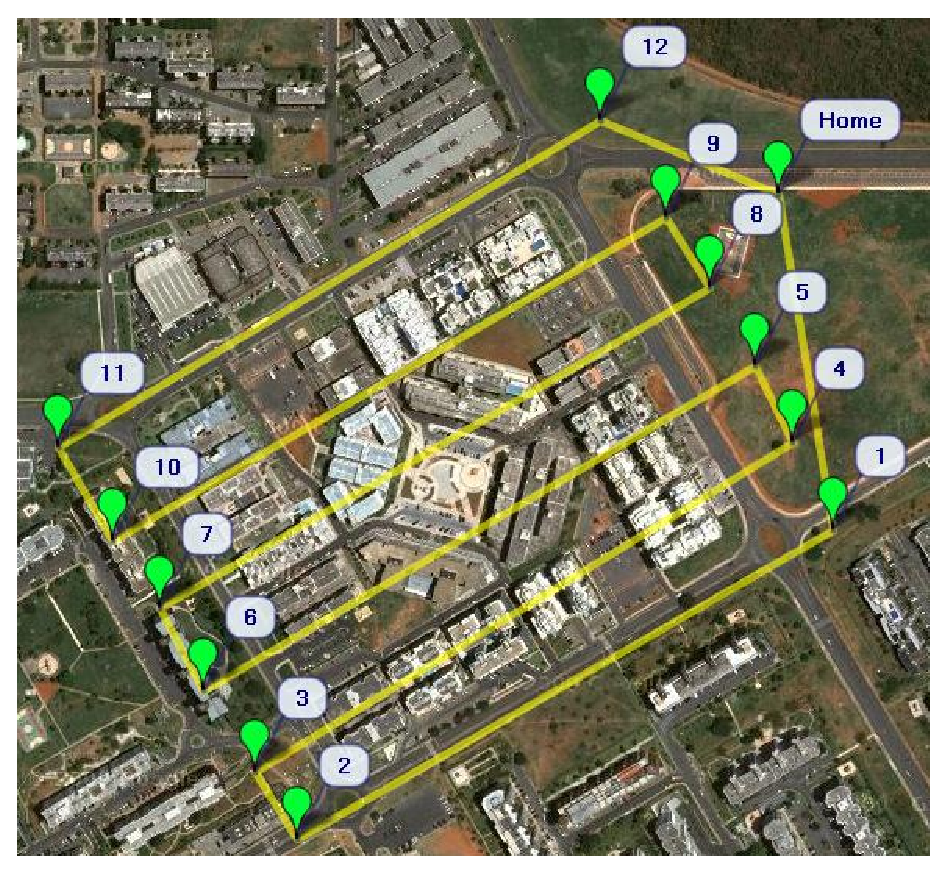
\includegraphics[width=3.5in]{figuras/plano_voo}
  \caption{Exemplo de Plano de Voo do VANT}
  \label{fig:plano_voo}
\end{figure}

\section{Algoritmo SIFT}

O algoritmo SIFT - Scale Invariant Feature Transform foi desenvolvido por [1] em 1999 e sua função é construir descritores de pontos-chaves de uma imagem, sendo este descritores independentes das mudanças de escala, rotação, translação e luminosidade que uma imagem pode sofrer. Utilizamos neste trabalho a implementação em C++ obtida em \cite{vedaldi}.
O SIFT é utilizado na busca por correspondências entre sequência de imagens diferentes que contenham partes da mesma cena. A busca é feita através de pontos-chave correspondentes, utilizando-se seus descritores. Nesta pesquisa a distância euclidiana é utilizada em três abordagens diferentes para avaliar a mais apropriada para imagens obtidas por VANTs. Os algoritmos de cada abordagem são: DistEuclidConvencional, o qual aplica a função de busca diretamente, sem tratar seus resultados. DistEuclidRedundante, que chama a função de busca duas vezes, a segunda chamada é feita invertendo-se os parâmetros da função, somente correspondências que ocorram em ambas são guardadas. DistEuclidEsc onde observa-se a continuidade de escala entre segmentos de reta traçados entre os pontos pertencentes e às correspondências geradas por esta função.

% \begin{figure}[!t]
%  \centering
%  \includegraphics[width=3.5in]{figuras/fluxograma}
%  \caption{Fluxograma do Programa}
%  \label{fig:fluxograma}
% \end{figure}

\clearpage

\section{Transformadas Geométricas}
( texto do Juliano )

\section{ Fluxograma para gerar o Mosaico}
 A montagem do mosaico se baseia em duas classes do Terralib, o arquivo MMIOMatching recebe duas imagens e apresenta como resultado os pontos de controle da cena, que são representados através de dois vetores para calculo da função de transformação. Esses pontos localizados são acrescentados na imagem que é salva com outro nome.
(Talvez colocar algo da dissetação do Dmitri Fedorov)
 Já o segundo arquivo  Mosaic recebe como entrada  a saida do  arquivo MMIOMatching, ou seja, os vetores  que representam os pontos de controle, além das imagens que serão mosaicadas e o nome da nova imagem.
(Devemos definir as configurações nesse item, qual foi a função de transformação que usamos entre outros detalhes, seria interessante fazer um desenho com explicando esse clico)

\section{Resultados}
Devemos descrever quanto tempo levou para executar, quantas imagens foram utilizadas para gerar o mosaico, quais as vantagens. 

\section{Comparação dos algoritmos}
Comparação do SIFT e dos algoritmos do Terralib

\section{Conclusão}
Conclusão aqui.

\begin{thebibliography}{1}

\bibitem{canhoto}
A.~Canhoto, E.~H.~Shiguemori, M.~A.~P.~Domiciano, \emph{Image sequence processing applied to autonomous aerial navigation}. Signal and Image Processing Applications, 2009. Proceedings ... Kuala Lumpur, Malasia: IEEE,
2009. p. 496-499.

\bibitem{goltz1}
G.~A.~M.~Goltz, E.~H.~Shiguemori, \emph{Aplicação do Algoritmo SIFT em Imagens de Navegação Autônoma}. In:
Workshop Anual de Pesquisa e Desenvolvimento do IEAv. São José dos Campos: IEAv, 2008. p. 35.

\bibitem{lowe}
David~G.~Lowe, \emph{Distinctive image features from scale-invariant keypoints}. International Journal of Computer Vision, 60, 2 (2004), pp. 91-110. Disponível em: <http://www.cs.ubc.ca/~lowe/papers/ijcv04.pdf>. Acesso em 20 de Dezembro de 2011.

\bibitem{vedaldi}
A.~Vedaldi, \emph{SIFT++: A Lightweight C++ implementation of SIFT}. Disponível em: <http://www.vlfeat.org/~vedaldi/code/siftpp.html>. Acesso em 20 de Dezembro de 2011.

\bibitem{gonzalez}
R.~C.~Gonzalez; R.~E.~Woods, \emph{Processamento de Imagens Digitais}. 3.~ed.\hskip 1em plus 0.5em minus 0.4em\relax São Paulo, Brasil: Edgard Blucher, 2010.

\bibitem{schowengerdt}
R.~A.~Schowengerdt, \emph{Remote Sensing: Models and Methods for Image Processing}. 2nd~ed.\hskip 1em plus 0.5em minus 0.4em\relax  Elsevier Inc, 2007.

\bibitem{jose}
C.~G.~José, E.~H.~Shiguemori, \emph{Processamento de imagens obtidas com diferentes ângulos de visada para aplicação na navegação autônoma}. Seminário Anual de Iniciação Científica e Pós-Graduação do IEAv, 4. Anais ... São José dos Campos, Brasil: IEAv, 2010. v. 1, p. 61-62.

\bibitem{goltz2}
G.~A.~M.~Goltz, \emph{Redes neurais artificiais em imagens para estimação da posição de um VANT}; São José dos Campos : INPE, 2011

\end{thebibliography}

\end{document}
